\section{Experiment}
\label{sec:experiment}
% a simple tool for multiple choice dataset evaluation and correction

We proceed to demonstrate the utility of our framework in three aspects:
 First, we use our method to evaluate 12 datasets which are from 6 different tasks 
 which are shown in~\figref{fig:datasets_exp}. 
 Second, we will test the deviation of different models on our split test datasets 
 in which contain easy and hard part. 
 Third, we filter out higher quality datasets to investigate if training on filtered dataset can 
 improve models' performance on hard test.
%\KZ{Give a table of the basic stats of these datasets? Why 1 less than yesterday?
%Also give the models for each the datasets in another table to give ppl a birds eyes view.} 
 
 %\end{itemize}

\begin{figure*}[h]
\centering
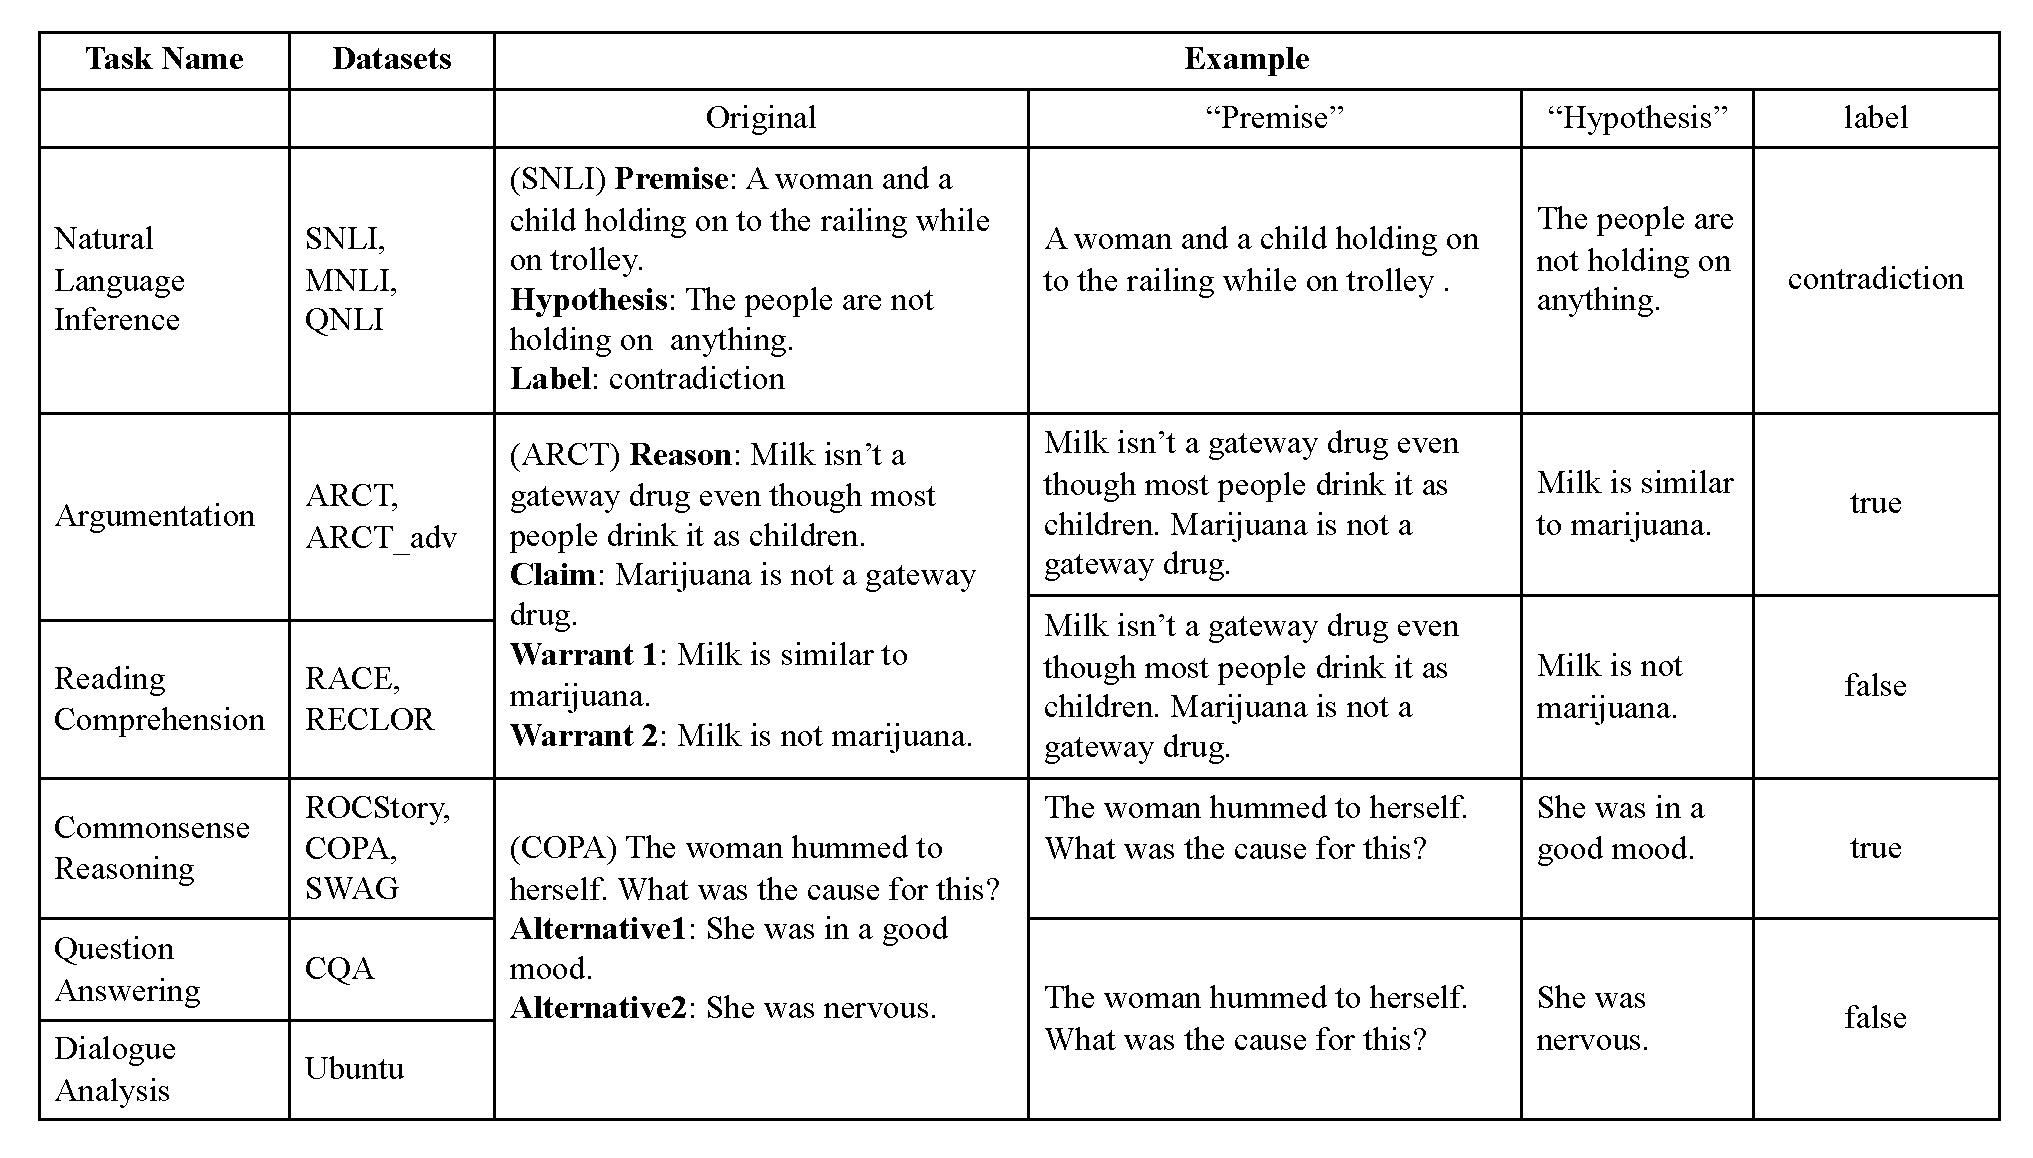
\includegraphics[width=2\columnwidth]{picture/datasets_exp.eps}
\caption{Data examples and normalized version.}
\label{fig:datasets_exp}
\end{figure*}

 \subsection{Our results on different tasks}
 \label{sec:experiment1}
 
 We experiment on 12 datasets in \figref{fig:datasets_exp}. 
 %These datasets are widely used in their 
 %respective fields to provide relevant knowledge and evaluate whether 
% models have the ability to solve the the problems in a field. %
%We have give some examples in \figref{fig:datasets_exp}. 
These datasets can mainly be classified into two types of tasks. 
The first type are the NLI classification tasks, a special case of multiple choice datasets. 
The second type are the multiple choice problems, including ARCT, 
ARCT\_adv\cite{schuster2019towards}, 
RACE~\cite{lai2017race}, and RECLOR~\cite{yu2020reclor}, in which ``hypothesis'' 
is one of the alternatives and ``premise'' contains more than one context roles. 
%\KZ{Don't understand: only has the premise and the hypothesis without the choices.}
For example, in~\figref{fig:datasets_exp}, 
ARCT dataset have \textbf{Reason} and \textbf{Claim} as ``premise'' 
which requires to select the right warrant between them. 
%The alternative warrant is the hypothesis and the premise is consist of  reason and claim. 
%RACE and Reclor includes context and questions which will be seen as ``premise''. 
%The label for each alternative is 
%``true'' or ``false'' for whether this hypothesis is the correct one.
Ubuntu~\cite{lowe2015ubuntu}, COPA~\cite{roemmele2011choice}, ROCStory, SWAG~\cite{zellers2018swag} and 
CQA~\cite{talmor2019commonsenseqa} also belong to the second type but with only context role 
in ``premise''.
Moreover, In \tabref{dataset_intro}, we 
show the hypothesis collection methods of these datasets. The hypothesis 
in most of datasets are written by human, except for CQA and SWAG. And only two of
them have adversarial experiments to amend the datasets.    
 
\begin{table}[h]
\scriptsize
\centering
\begin{tabular}{p{7mm}cccccc}\hline
\textbf{Datasets} &Data Size & Data source& AE& Human(\%)\\ \hline                                   
ROCStory & 3.9k         & CD         &No    &100.0  \\
COPA        & 1k           &  CD           &No   &100.0     \\
SWAG       & 113k       &  LM            &Yes  & 88.0\\
SNLI          &  570K     & CD           &No     &80.0\\
QNLI         & 11k         &  CD            &No    &80.0\\
MNLI         & 413k       &  CD            & No   &80.0\\
RACE        & 100k      &  CD            &No    &94.5\\
RECLOR       &  6k          &  CD             &No   &63.0\\
CQA         & 12k        &  CD              &No    &88.9\\
ARCT         & 2k         & CD               &No    &79.8\\
ARCT\_adv& 4k         & CD                &Yes   & -\\
Ubuntu   & 100k      &Random Selection & No  & -  \\
\hline
\end{tabular}
\caption{\label{dataset_intro} The hypothesis collection methods of datasets.  
AE = Adversarial Experiment, LM = language model, CD = crowdsourcing, Human represents 
human performance on the datasets}
\end{table}
 
To  show if the unigram and cross-unigram cues really exist in these datasets, 
we use diverse metrics (in~\secref{sec:approach}) to get cue features. 
Then we use the simplest ways, the average value classifier(AveC), 
the maximum value classifier(MaxC), SGD classifier(SGDC) and 
logistic regression(LR) (\secref{sec:approach}), 
to make decision about choices only with the spurious statistical features. 

\begin{table}[th]
\scriptsize
\centering
\begin{tabular}{p{7mm}cccccc}\hline
\textbf{Datasets} &Random & \multicolumn{2}{c}{Unigram Cues} &  \multicolumn{2}{c}{Cross-unigram Cues} \\ \hline
                                     & (\%)                 &  Acc.(\%) & $\mathcal{D}(\%)$&  Acc.(\%) & $\mathcal{D}(\%) $ \\ \hline         
ROCStory & 50.0            & 68.68          & \textbf{18.68}                    &70.92          & \textbf{20.92}\\
COPA        & 50.0           & 55.60           &  5.60                   &53.60          & 3.60 \\
SWAG       & 25.0           & 27.23           &   2.23                  &33.56          & 8.56\\
SNLI          & 33.33      & 62.57           &  \textbf{29.24}                  &66.92         & \textbf{33.59}\\
QNLI         & 50.0           & 62.49            &  \textbf{12.49}                 &64.93          &\textbf{14.93}\\
MNLI         & 33.33      & 51.37            &\textbf{18.04}                 &51.84          & \textbf{18.50} \\
RACE        & 25.0          & 35.42            &   \textbf{10.42}                 &39.68          &\textbf{14.68}\\
RECLOR       & 25.0           & 34.80            &   9.80                  &39.20           &\textbf{14.20}\\
CQA          &20.0            & 23.42            &  3.42                   &22.85           &  2.85\\
ARCT        & 50.0            & 54.95           &  4.95                  & 53.38          & 3.38\\
ARCT\_adv& 50.0           &50                 &0.0                     & 51.46            & 1.46 \\
Ubuntu   & 1.0               &4.96              &3.96                     &3.74          &2.74\\
\hline
\end{tabular}
\caption{\label{best_acc} Highest accuracy of our 4 simple classification models
on 12 datasets and the deviations from random selection}
\end{table}

In order to measure the degree of statistical features in data sets, we propose to use the 
deviation from the random selection probability as a measurement which can be expressed as:

\begin{equation}
    \mathcal{D} = {Acc}_{cue}  -
    {Random}
\end{equation}

${Acc}_{cue} $ represents the performance of a model which based on cue features only. 
And ${Random}$ is the accuracy with random selection. 
$\mathcal{D}$ measures how heavy the cue patterns ``leak'' from training 
data to testing  data. ``Leakage'' here means the same cue distribution exists in both training 
and testing data. 
%The cues are patterns with bias feature ``leakage'' which has been introduced in~\secref{sec:intro}.
Obviously, the higher absolute value of $\mathcal{D}$ suggests 
the larger amounts of cues existing in a dataset. The opposite, that is, smaller $\mathcal{D}$
doesn't mean there is fewer spurious cues, but less ``leakage''. 
The cues can be different between training and testing dataset.
If $\mathcal{D}$ is positive, it means the 
cues can help to make the right choice. Otherwise, it indicates that the dataset is harder with
inconsistent statistical cues.  This evaluation method 
can estimate any collected multiple choice dataset. 
For providing  a high quality stress test dataset, 
%the first condition is that it's hard to 
%choose right choice with ``leakage'' feature only. In another word, 
it's important to break the ``leakage'' 
between them.

%\begin{table*}[th]
% \scriptsize
%\centering
%\begin{tabular}{p{10mm}cccc|cccc|cccc}\hline
%\textbf{Datasets} & \multicolumn{4}{c|}{Top1} & \multicolumn{4}{c|}{Top2} &  \multicolumn{4}{c}{Top3} \\ \hline
%                           & \multicolumn{2}{c}{Unigram} &  \multicolumn{2}{c|}{Cross-unigram}&  \multicolumn{2}{c}{Unigram} &  %\multicolumn{2}{c|}{Cross-unigram}& \multicolumn{2}{c}{Unigram} &  \multicolumn{2}{c}{Cross-unigram}\\ \hline   
%                           &Metric &Method  &Metric &Method &Metric &Method &Metric &Method &Metric &Method &Metric %&Method \\ \hline    
%ROCStory  &RF&LR & CP&LR     &    CP&LR &RF&LR      &RF&SGDC&PMI&LR\\
%SNLI          &PMI&LR& PMI&LR   &    CP&LR  &CP&LR     &CP&SGDC&RF&LR\\
%QNLI         &Freq&LR& CP&LR    &    CP&LR  & CP&AveC           &PMI&LR  &PMI&AveC \\
%MNLI         &CP&LR  &CP&LR     &     PMI&LR & CP&SGDC         &CP&SGDC &RF&LR\\
%RACE        & CP&LR &CP&LR     &    CP&SGDC & PMI&LR          &PMI&LR& RF&LR\\
%RECLOR      & Cos&LR &CP&LR     &   Cos&SGDC  & RF&LR      &CP&LR&  Cos&LR\\
%\hline
%\end{tabular}
%\caption{\label{best_method} Top three corresponding metrics and 4 simple classification methods of accuracy ranking on different datasets.}
%\end{table*}


\begin{table}[th]
 \scriptsize
\centering
\begin{tabular}{p{7mm}ccccc}
\hline
Method & Metric & \multicolumn{2}{c}{Unigram} &  \multicolumn{2}{c}{Cross-unigram}\\ \hline    
            &              & Num. & \%& Num.& \%\\ \hline    
LR&CP&  6 & 100& 6& 100 \\
LR&PMI  &4&66.67& 3 &50.0\\
LR&RF&  1 &  16.67&5& 83.33\\
SGDC&CP&3&50.0&1&16.67\\
LR&Freq &1&16.67&0&0.0\\
LR&Cos  & 1&16.67&1&16.67\\
SGDC&RF&1&16.67&0&0.0\\
SGDC&Cos&1&16.67&0&0.0\\
AveC&CP&0&0.0&1&16.67\\
AveC&PMI&0&0.0&1&16.67\\ \hline
\end{tabular}
\caption{\label{best_method} Test cue metrics and aggregation methods with unigram and cross-unigram cue features on six data sets. It's the number and proportion of accuracy ranking in the top three (the max number must be six because there are only six data sets)}
%The number and percentage for different methods and metrics in top three with the accuracy on  6 datasets.}
%classification methods of accuracy ranking on different datasets.}
\end{table}

In \tabref{best_method}, the selection
%\KZ{Don't use such emotional terms: absurd} 
results through statistical cues features only on several datasets are striking, 
for example the highest accuracy with our methods for ROCStories dataset 
substantially exceeds the random selection probability by 20.92\% and even higher  for SNLI dataset 
by 33.59\%.  As was expected, 
manually intervened datasets without adversarial experiment 
for filtering contain more spurious statistical cues. 
The result for ARCT\_adv which adjust ARCT dataset by human does have a certain effect (from 54.95\% to 50\%).
But how deviation $\mathcal{D}$ identifies which datasets are seriously problematic? 
Based on our experience, if $\mathcal{D}$ of a models beyond 10\% on either cue feature, this model will be 
determined as a problematic dataset.
%statistical cues problem.we define the boundaries 
%for this purpose on 10\%. 
In~\tabref{best_method}, we consider 
ROCStories, SNLI, MNLI, QNLI, RACE and RECLOR are the datasets containing heavier
statistical cue problem. 6 out of 12 datasets are ``bad'' datasets which 
indicates unigram and cross-unigram 
cues are general problems for multiple choice datasets. 


 Now, there is still a question that which cue metric can better represent cue features 
 and which method is proper to aggregate the cue features 
 for exploring the weaknesses in the datasets. We have 8 cue metrics and 4 aggregation 
 methods to select the choices. Trying on all permutation, we can choose the 
 best one which can get high accuracy on 6 datasets all the time. 
 The number of the combination cue metrics and methods that can get the accuracy in top 3 of 
 different datasets are shown in~\tabref{best_method}. (detailed scores for all permutation are recorded
in Appendix).
 %, top three corresponding metrics and classification methods of accuracy ranking on problematic 
 %datasets we mentioned above. in~\tabref{best_method}, 
 %By observing the results,
 It is apparent that  the conditional probability(CP) with logistic regression(LR) is 
 most likely to fully utilize cues for getting the best results. Its performance is in top 3 
 for all 6 datasets. Meanwhile, 
 CP, Freq, PMI, RF and Cos are better to measure the degree of unigram related cues then LMI 
 and WP which also consider the term frequency. It indicates that the low frequency but 
 highly unbalanced tokens can also influence the decision heavily. 
 We can deem that cue features has relatively small 
 relationship with frequency. It is noted that we will only use CP metric and LR 
 method to get spurious feature and split datasets.
 
 
 We have shown to what extent a dataset 
 contains unigram or cross-unigram cues by deviation $\mathcal{D}$. The original datasets are 
 automatically be separated into easy and hard part that is determined by whether the instance 
 can be correct chosen or not.
 Moreover, it is suspicious that whether the models really learn these features 
 to make good performance or not. We will explore more in the following sections.
 
 
\subsection{Performance Gap on Easy and Hard Part}
\label{sec:experiment2}
%\KZ{Instead of deviation, call it ``performance gap''?}
If a model learns the cue features in a dataset, It 
 will probably make a tendentious choice on 
 test set according to the samples whether have same cue features or not. 
 Thus we make an assumption that if a model is affected by cues 
in the dataset, it will have different performance on easy and hard parts 
we have 
 separated in~\secref{sec:experiment1}.
 %only divided by the extent to spurious cues. 
 The deviation between the results on each part can be called \textbf{performance gap} 
 which shows the robustness of the model. %We call it robustness, because 
 If a model 
 can really capture the ability to solve the problem, it will not be easily attracted by 
 the spurious information and will have resemble performance on both easy and hard 
 part. Besides, the performance on hard part is also an importance criteria that
 can indicate the capability of models.

\begin{table*}[th]
\scriptsize
\centering
\begin{tabular}{c|c|llll|lll|lll}
Dataset                                      & \multicolumn{1}{c|}{Model} & \multicolumn{1}{c|}{Original} & \multicolumn{3}{c|}{Unigram}                                                                  & \multicolumn{3}{c|}{Cross-unigram}                                                            & \multicolumn{3}{c}{\textbf{Combination}}                                                                  \\ \hline
                                             &                            & \multicolumn{1}{c|}{(\%)}      & \multicolumn{1}{c}{Easy (\%)} & \multicolumn{1}{c}{Hard (\%)} & \multicolumn{1}{c|}{\textbf{gap} (\%)} & \multicolumn{1}{c}{Easy (\%)} & \multicolumn{1}{c}{Hard (\%)} & \multicolumn{1}{c|}{\textbf{gap} (\%)} & \multicolumn{1}{c}{Easy (\%)} & \multicolumn{1}{c}{Hard (\%)} & \multicolumn{1}{c}{\textbf{gap}(\%)} \\ \hline
\multicolumn{1}{c|}{\multirow{3}{*}{SNLI}}   & BERT                       & \multicolumn{1}{l|}{90.48}    & 94.99                         & 83.02                         & 11.97                         & 95.05                         & 81.31                         & 13.73                         & 94.40                         & 80.55                         & 13.85                        \\
\multicolumn{1}{c|}{}                        & ESIM                       & \multicolumn{1}{l|}{87.44}    & 93.27                         & 77.77                         & 15.50                         & 93.22                         & 75.83                         & 17.39                         & 92.57                         & 74.44                         & 18.13                        \\
\multicolumn{1}{c|}{}                        & fastText                   & \multicolumn{1}{l|}{54.74}    & 73.16                         & 24.23                         & 48.93                         & 69.92                         & 24.23                         & 45.69                         & 68.46                         & 20.02                         & 48.44                        \\ \hline
\multicolumn{1}{c|}{\multirow{3}{*}{MNLI}}   & BERT                       & \multicolumn{1}{l|}{85.10}    & 90.60                         & 79.30                         & 11.30                         & 90.27                         & 79.55                         & 10.72                         & 89.91                         & 77.04                         & 12.87                        \\
\multicolumn{1}{c|}{}                        & ESIM                       & \multicolumn{1}{l|}{76.82}    & 85.80                         & 67.34                         & 18.46                         & 85.51                         & 67.48                         & 18.03                         & 84.38                         & 64.15                         & 20.23                        \\
\multicolumn{1}{c|}{}                        & fastText                   & \multicolumn{1}{l|}{47.15}    & 66.88                         & 26.31                         & 40.56                         & 64.16                         & 28.86                         & 35.29                         & 61.74                         & 22.71                         & 39.03                        \\ \hline
\multicolumn{1}{c|}{\multirow{3}{*}{QNLI}}   & BERT                       & \multicolumn{1}{l|}{88.89}    & 90.92                         & 85.54                         & 5.37                          & 90.97                         & 85.01                         & 5.96                          & 90.44                         & 84.07                         & 6.37                         \\
\multicolumn{1}{c|}{}                        & ESIM                       & \multicolumn{1}{l|}{72.17}    & 78.55                         & 61.66                         & 16.89                         & 77.86                         & 61.57                         & 16.29                         & 76.57                         & 58.57                         & 18.00                        \\
\multicolumn{1}{c|}{}                        & fastText                   & \multicolumn{1}{l|}{66.33}    & 80.94                         & 42.26                         & 38.67                         & 77.19                         & 46.08                         & 31.11                         & 76.08                         & 36.14                         & 39.94                        \\ \hline
\multicolumn{1}{c|}{\multirow{3}{*}{ROC}}    & BERT                       & \multicolumn{1}{l|}{90.54}    & 93.53                         & 84.01                         & 9.52                          & 93.67                         & 82.90                         & 10.77                         & 93.24                         & 82.00                         & 11.24                        \\
\multicolumn{1}{c|}{}                        & ESIM                       & \multicolumn{1}{l|}{65.42}    & 72.49                         & 50.00                         & 22.49                         & 73.02                         & 46.88                         & 26.15                         & 71.99                         & 44.67                         & 27.32                        \\
\multicolumn{1}{c|}{}                        & fastText                   & \multicolumn{1}{l|}{62.91}    & 71.16                         & 44.90                         & 26.26                         & 72.34                         & 39.89                         & 32.45                         & 70.44                         & 39.11                         & 31.33                        \\ \hline
\multicolumn{1}{c|}{\multirow{3}{*}{RACE}}   & BERT                       & \multicolumn{1}{l|}{90.54}    & 93.53                         & 84.01                         & 9.52                          & 93.67                         & 82.90                         & 10.77                         & 93.24                         & 82.00                         & 11.24                        \\
\multicolumn{1}{c|}{}                        & ESIM                       & \multicolumn{1}{l|}{65.42}    & 72.49                         & 50.00                         & 22.49                         & 73.02                         & 46.88                         & 26.15                         & 71.99                         & 44.67                         & 27.32                        \\
\multicolumn{1}{c|}{}                        & fastText                   & \multicolumn{1}{l|}{62.91}    & 71.16                         & 44.90                         & 26.26                         & 72.34                         & 39.89                         & 32.45                         & 70.44                         & 39.11                         & 31.33                        \\ \hline
\multicolumn{1}{c|}{\multirow{3}{*}{RECLOR}} & BERT                       & \multicolumn{1}{l|}{48.40}    & 61.68                         & 41.74                         & 19.93                         & 63.78                         & 38.49                         & 25.29                         & 60.52                         & 37.83                         & 22.69                        \\
\multicolumn{1}{c|}{}                        & ESIM                       & \multicolumn{1}{l|}{40.40}    & 52.69                         & 34.23                         & 18.46                         & 52.04                         & 32.89                         & 19.15                         & 50.64                         & 31.46                         & 19.18                        \\
\multicolumn{1}{c|}{}                        & fastText                   & \multicolumn{1}{l|}{31.60}    & 43.11                         & 25.83                         & 17.29                         & 40.82                         & 25.66                         & 15.16                         & 39.06                         & 25.09                         & 13.96                        \\ \hline
\end{tabular}
\caption{\label{best_acc} The performance gap on easy and hard test dataset for models. 
Models capture unigram, cross-unigram or the combination as cue features to make decision}
\end{table*}


We evaluate the the performance of 3 typical models, 
BERT~\cite{devlin2018bert}, ESIM~\cite{peters2018deep} and fastText~\cite{joulin2017bag} , 
which represent different levels of complexity on the 6 ``bad'' datasets respectively:

\textbf{fastText} models sentences as a bag of n-grams, and tries to predict
the probability of each answer being correct independently. The representation of 
tokens are from GloVe embeddings with 300 dimension. We select the answer with the highest
score as the prediction for the multiple-choice setting.

\textbf{ESIM}(Enhanced Sequential Inference Model) 
A method that introduces local inference modeling,
which models the inference relationship between
premise and hypothesis after the two fragments aligned
locally. We train our own ESIM model
with GloVe embeddings.  We also choose the answer with the highest
score.

\textbf{BERT} exploits transformer~\cite{vaswani2017attention}
block  which is a popular basic computational unit. BERT is
is trained on BooksCorpus~\cite{zhu2015aligning} and English Wikipedia in two unsupervised
tasks, i.e., Masked LM (MLM) and Next Sentence Prediction (NSP). 
There are several available pre-trained BERT models which differ in how
many layers and parameters are used in the mode. 
We choose to use the basic one with 12-layer transformer blocks, 768 hidden-size, and 12 self attention
heads, totally 110M parameters 
and fine-tune for 3 epochs to predict
the relation based on the concatenation of the
premise and hypothesis (with a delimiter token).

The performance of these models on different datasets are shown in \tabref{best_acc}. 
The gap between easy and hard parts typical ranges from 10-50\%. 
In contrast, humans can still keep good performance on hard set which shows that 
these models may all influenced by the statistical cues to some extent in each dataset. 
The ``combination'' means we aggregate the choice made by unigram and cross-unigram cues.
The easy part for ``combination'' is the union of easy parts of the other two cue features and 
the hard part is the intersection of two other hard parts. And we can find the ``combination'' mostly take deeper 
gap.

If we compare the gaps among the three models, 
we can find that BERT, ESIM and fastText have increasingly larger gaps.
The huge gap for fastText 
%is heavily affected by the split of test set 
suggests that the simple 
structure is more easily be affected by cue features.
%a model driven by
%token level features and leave out 
%and our split strategy is also based on unigram tokens.
%The fact that fastText is worse than random guess on the hard part shows that
%it is not really understanding the text beyond simple word correlations.
BERT may be more robust than the other two models. However, it's gaps on 6 datasets 
are all beyond 10\% which indicates BERT is also suffer from the cues. Moreover, the model with 
highest score may not always be the most stable one. On the last two rows for RACE and RECLOR 
datasets, though BERT has higher accuracy on the whole and hard dataset, 
the gap is higher than other models. The gap of ESIM on RACE is small, but it doesn't  
indicate ESIM is better without considering the performance on hard test data which 
is close to random selection. 
It can be difficult for ESIM to converge on RACE and RECLOR
datasets. 
In general, we should consider the accuracy and the robustness 
synthetically. We provide an efficient way to evaluate the models with a new ``stress test'', hard data test. 

% \subsection{Improve the performance of models with dataset filtering}
\subsection{Toward better model robustness by filtering training data}
\label{sec:experiment3}
%Following previous sections where we showed that some statistical spurious cues existing 
%in many datasets. These cues 
%can misleading the model to focus on shallow spurious features and 
%reduced the stability of the models. We split the test datasets which 
%have heavy ``leakage" problems with its training data by breaking the dependency on the tokens’ distribution. 
%
Previously we managed to split the test set into easy and hard part using
the simple LR model trained with the original training data.
One question arises that whether it is possible to ``split'' the training
data in the same way and use the hard part of the training data to
train a better, more robust neural model?
We achieved this by firstly doing an $n$-fold random split on the training
data, then training the LR model from $n-1$ parts and testing it on the
last part in a round-robin fashion.
For simplicity, we only used the combined feature to train the LR model. 
After $n$ rounds, we will get the easy-hard split on the whole
training data. We call the hard part the ``filtered'' training data
as opposed to the original training data. 
Will the filtered training data help us train a better model?

In our next experiment, we train BERT, ESIM and fastText models
on the filtered training data of the six ``bad'' datasets, 
and compare the accuracies on hard part of the test data with the previous accuracies
using the original training data. 
Results are shown in \tabref{tab:filtered}. 

%the same spurious cues or not. However, different with dataset evaluation which requires  the least ``leakage'' 
%between training and testing, a high quality training data demands few spurious cues which can misleading the model and 
%we wonder
%that whether the left part which can not be correct chosen by LR model  is balanced without any cues 
%or just have other bias features which 
%are conflict to the original part. 
%Thus we split the training datasets with n-fold test and follow the method of splitting 
%test datasets(~\secref{sec:approach}). 
%We use combination 
%of unigram and cross-unigram features to 
% separate the samples.
%There are two possible outcomes:
%%If we can find that the part with less ``leakage'' 
%First, if the gap between the easy and hard test datasets is smaller, 
%it may indicates that the ``filtered part'' 
%is more balance than original datasets.
%Second, if the absolute gap is larger, it can suggest that the 
%``filtered part'' may contain other features different from original 
%test datasets. 

\begin{table}[th]
\scriptsize
\centering
\begin{tabular}{p{5mm}ccccccc}
&    & SNLI & MNLI & QNLI & ROC & RACE & RECLOR \\ \hline
\multirow{2}{*}{BERT} &O& 80.55& 77.04 & 84.07 & 82.00 & 54.31& 37.83 \\ 
                      &F& \textbf{87.53} & \textbf{82.25} & \textbf{86.14} & \textbf{86.40} &\textbf{55.48} & 37.82 \\ \hline
\multirow{2}{*}{ESIM} &O& 74.44 & 64.15 & 58.57  & 44.67 &28.14 & 31.46 \\ 
		&F& 67.43 & 54.24 & \textbf{64.43} & \textbf{50.0} & \textbf{28.85} &30.34   \\ \hline
\multirow{2}{*}{fastText} &O& 20.02 & 22.71& 36.14 & 39.11 & 21.05& 25.09\\
                          &F & \textbf{47.45}&  \textbf{45.90} & \textbf{69.92}& \textbf{55.78} & \textbf{27.04} & \textbf{30.71} \\ \hline
\end{tabular}
\caption{\label{tab:filtered} Improving the Robustness of Models on the Hard Test Sets using
Filtered Training Data. O: Original, F: Filtered.}
\end{table}

We find that except for ESIM on the three NLI datasets, all models show better performance
on all datasets (bolded numbers), sometimes by very large margin ($>20\%$). We speculate that the models thus
learned have disregarded the simple token-level cues (because there are fewer of them in the filtered training data now) and turned to focus more on other more meaningful and perhaps more sophisticated features. 
But whether the models are indeed more robust and closer to human reasoning remains to be seen. 
Because it could be that there are other cues what we cannot detect and filter in
the hard part, and now there is information leak between the train and test on these cues. 
Further investigate is needed as future work.
%\begin{table*}[th]
%\scriptsize
%\centering
%\begin{tabular}{ccccccccccc}
%                          & \multicolumn{1}{c|}{}         & \multicolumn{3}{c|}{SNLI}                                                 & \multicolumn{3}{c|}{MNLI}                                                 & \multicolumn{3}{c|}{QNLI}                                          \\ \hline
%                          & \multicolumn{1}{c|}{}         & easy                 & hard                 & \multicolumn{1}{c|}{gap}    & easy                 & hard                 & \multicolumn{1}{c|}{gap}    & easy                 & hard                 & gap                  \\
%\multirow{2}{*}{BERT}     & \multicolumn{1}{c|}{original} & 95.05                & 81.31                & \multicolumn{1}{c|}{13.73}  & 90.27                & 79.55                & \multicolumn{1}{c|}{10.72}  & 90.97                & 85.01                & 5.96                 \\
%                          & \multicolumn{1}{c|}{filtered} & 53.56                & 87.53                & \multicolumn{1}{c|}{-33.97} & 76.59                & 82.25                & \multicolumn{1}{c|}{-5.66}  & 66.0                 & 86.14                & -26.14               \\ \hline
%\multirow{2}{*}{ESIM}     & \multicolumn{1}{c|}{original} & 93.22                & 75.83                & \multicolumn{1}{c|}{17.39}  & 85.51                & 67.48                & \multicolumn{1}{c|}{18.03}  & 77.86                & 61.57                & 16.29                \\
%                          & \multicolumn{1}{c|}{filtered} & 37.51                & 61.22                & \multicolumn{1}{c|}{-23.71} & 60.28                & 54.94                & \multicolumn{1}{c|}{5.34}   & 27.51                & 55.26                & -27.75               \\ \hline
%\multirow{2}{*}{fastText} & \multicolumn{1}{c|}{original} & 69.92                & 24.23                & \multicolumn{1}{c|}{45.69}  & 64.16                & 28.86                & \multicolumn{1}{c|}{35.29}  & 77.19                & 46.08                & 31.11                \\
%                          & \multicolumn{1}{c|}{filtered} & 18.36                & 41.46                & \multicolumn{1}{c|}{-23.10} & 21.64                & 38.90                & \multicolumn{1}{c|}{-17.26} & 26.43                & 58.66                & -32.29               \\ \hline
%\end{f}
%\caption{\label{tab:filtered} Performance gap comparison between original datasets and filtered datasets}
%\end{table*}

